\documentclass{beamer}
\usetheme{BauhausNeuralFEM} 
\usepackage{amssymb}


% --- Title info ---
\title[ Assembly \& Boundary Conditions]{From FEM to Neural Operators: Scientific Machine Learning for Computational Mechanics\\[0.4cm]}
\subtitle{ Assembly \& Boundary Conditions}
\author{Dr-Ing Jorge Alberto L\'{o}pez Zerme\~{n}o}
\date{}

\graphicspath {{Figures/}}

% --- Helpful macros ---
\newcommand{\R}{\mathbb{R}}
\newcommand{\bK}{\mathbf{K}}
\newcommand{\bU}{\mathbf{U}}
\newcommand{\bfvec}{\mathbf{f}}
\newcommand{\be}{\mathbf{e}}
\newcommand{\domain}{\Omega}
\newcommand{\boundary}{\Gamma}
\newcommand{\diri}{\Gamma_D}
\newcommand{\neum}{\Gamma_N}

\begin{document}

%====================
{
	\usebackgroundtemplate{
		\begin{tikzpicture}[remember picture,overlay]
			\node[opacity=0.25,inner sep=0pt] at (current page.center)
			{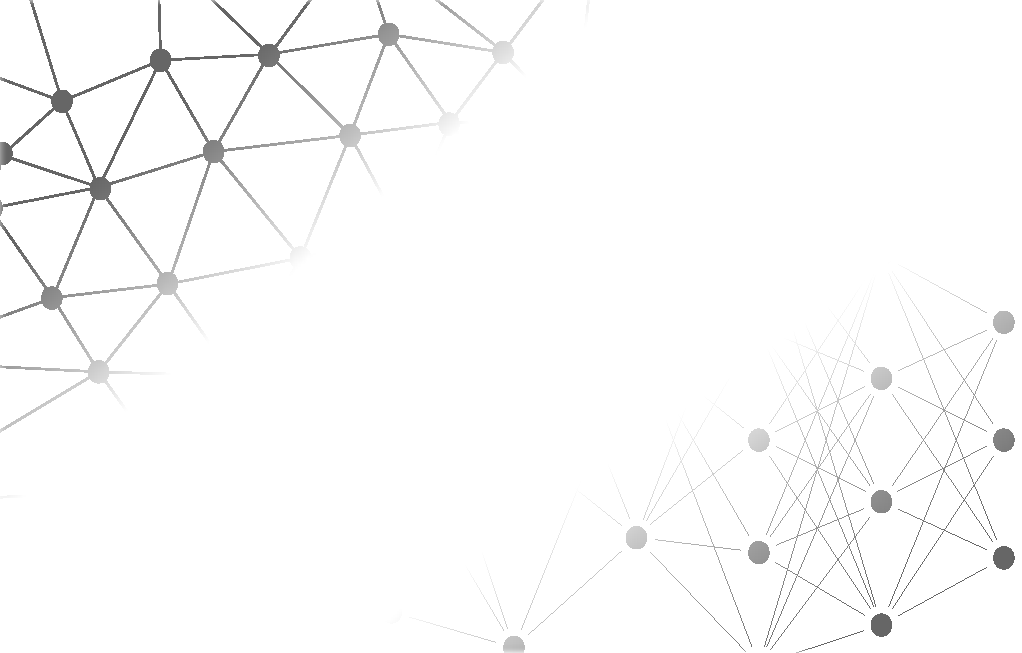
\includegraphics[width=\paperwidth,height=\paperheight]{Background.pdf}};
		\end{tikzpicture}
	}
	\begin{frame}[plain]
		\centering
		\begin{minipage}{0.21\textwidth}
			\centering
			
\includegraphics[width=\linewidth]{Bauhaus_Logo.png}
		\end{minipage}\hspace{105pt}
		\begin{minipage}{0.3\textwidth}
			\centering
			
\includegraphics[width=\linewidth]{JHU_Logo.png}
		\end{minipage}
		
		\titlepage
		\vspace{-35pt}
		Bauhaus Spring School 2026
		
	\end{frame}
}

%====================
\begin{frame}{Roadmap}
	\begin{minipage}{0.5\textwidth}
		\begin{center}
			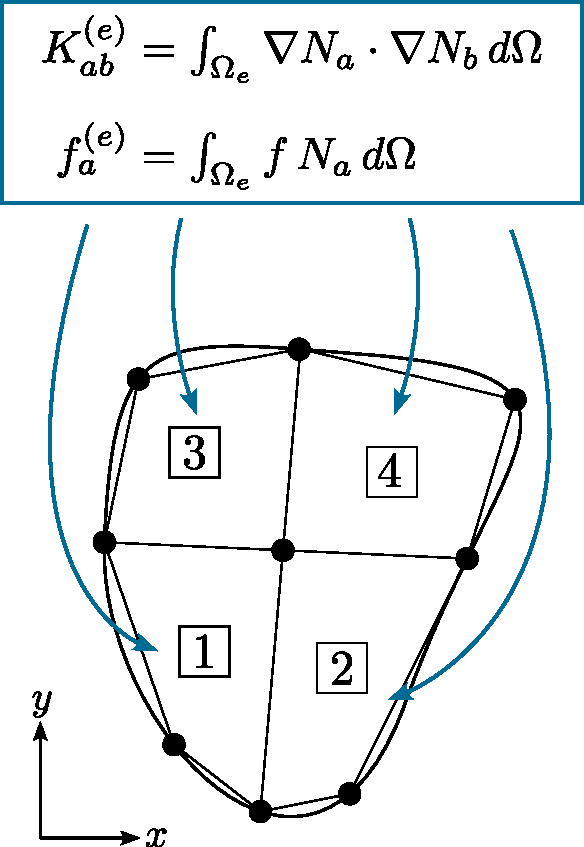
\includegraphics[width=0.85\linewidth]{Figures/Element_to_Global.pdf}
		\end{center}
	\end{minipage}\hfill
	\begin{minipage}{0.1\textwidth}
		\LARGE $\Rightarrow$
	\end{minipage}\hfill
	\begin{minipage}{0.35\textwidth}
		\begin{center}
		\small \textbf{Assembly:}
		\footnotesize
		\begin{equation*}
			\mathbf{K}\mathbf{u}=\mathbf{f}
		\end{equation*} 
		
		\LARGE $\Downarrow$
		
		\vspace{10pt}
		\small \textbf{Boundary Conditions:}
		\footnotesize
		\begin{equation*}
			\mathbf{K}\mathbf{u}=\mathbf{f}
		\end{equation*} 
		
		\LARGE $\Downarrow$
		
		\vspace{10pt}
		\small \textbf{Solution:}
		\footnotesize
		\begin{equation*}
			\mathbf{u}=\mathbf{K}^{-1}\mathbf{f}
		\end{equation*} 
	\end{center}
	\end{minipage}
	
\end{frame}


\begin{frame}{Element Connectivity and Assembly Operator}
	\begin{center}
		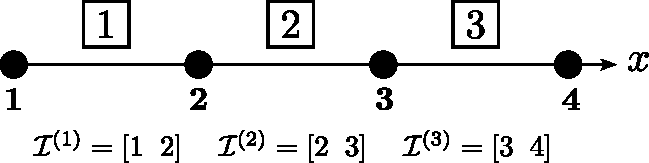
\includegraphics[width=0.48\linewidth]{Figures/IEN_1D.pdf}
	\end{center}
	\footnotesize
	\begin{itemize}
		\item \textbf{Element Connectivity Index:} $\mathcal{I}^{(e)} = \big(I^{(e)}_1,\dots,I^{(e)}_{n_e}\big)$
		
		\\
		$\rightarrow$ Global DOFs corresponding to element $e$
		
		\item  \textbf{Assembly Operator:}\\
		\vspace{-5pt}
		\begin{minipage}{0.6\textwidth}
			\[
			\mathcal{A}_e[\mathbf{K}^{(e)}]_{ij} 
			:= \sum_{a=1}^{n_e}\sum_{b=1}^{n_e}
			\big[\, i = \mathcal{I}^{(e)}_a \,\big]\,
			\big[\, j = \mathcal{I}^{(e)}_b \,\big]\,
			K^{(e)}_{ab}
			\]
			\[
			\mathcal{A}_e[\mathbf{f}^{(e)}]_i 
			:= \sum_{a=1}^{n_e}
			\big[\, i = \mathcal{I}^{(e)}_a \,\big]\,
			f^{(e)}_{a}
			\]
		\end{minipage}\hfill
		\begin{minipage}{0.32\textwidth}
			\begin{equation*}
				\mbox{where }
				[\cdot] \begin{cases}
					1\;\mbox{if true} \\
					0\;\mbox{otherwise}
				\end{cases} 
			\end{equation*}
		\end{minipage}
		
	\end{itemize}
	
	\begin{minipage}{0.33\textwidth}
		\begin{center}
			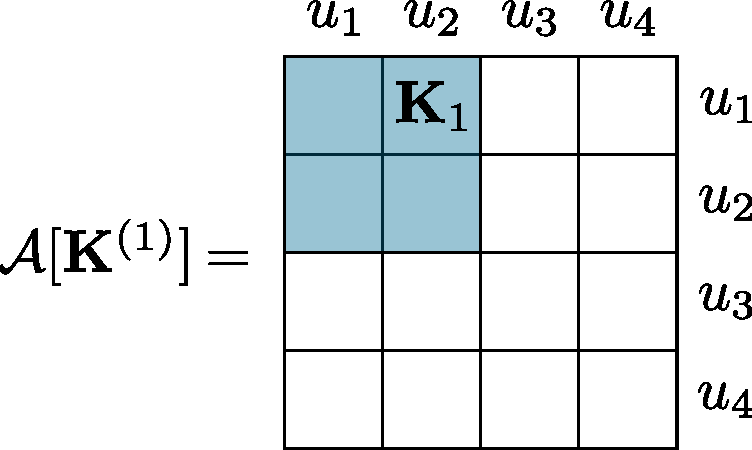
\includegraphics[width=0.96\linewidth]{Figures/Assembly_Operator_K1.pdf}
		\end{center}
	\end{minipage}\hfill
	\begin{minipage}{0.33\textwidth}
		\begin{center}
			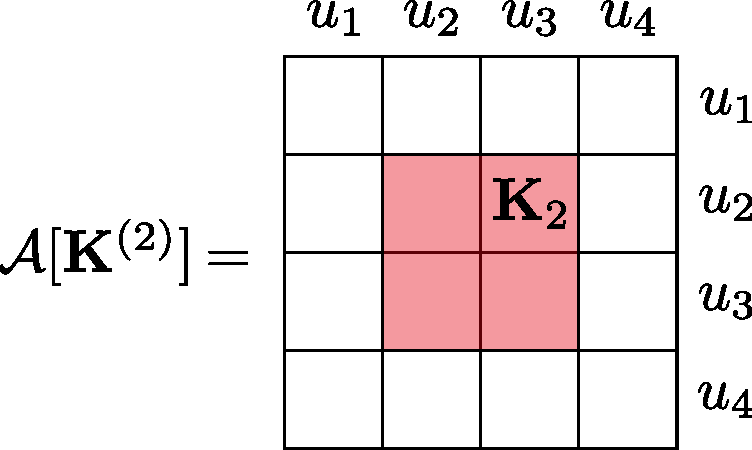
\includegraphics[width=0.96\linewidth]{Figures/Assembly_Operator_K2.pdf}
		\end{center}
	\end{minipage}\hfill
	\begin{minipage}{0.33\textwidth}
		\begin{center}
			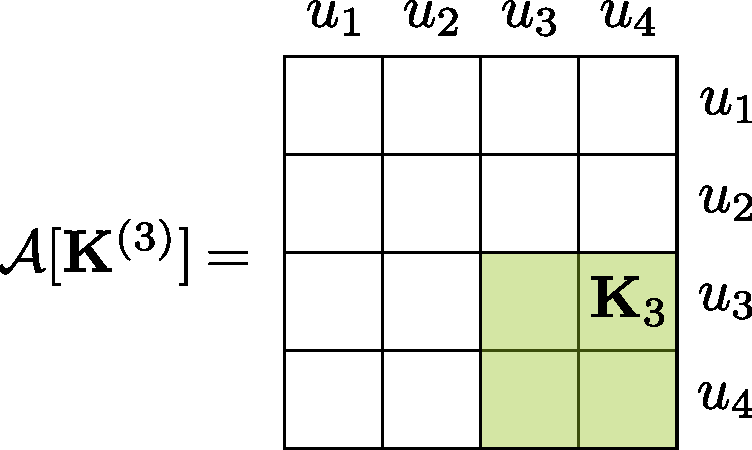
\includegraphics[width=0.96\linewidth]{Figures/Assembly_Operator_K3.pdf}
		\end{center}
	\end{minipage}

\end{frame}


%====================
\begin{frame}{Building the global system (1D)}
	\begin{center}
		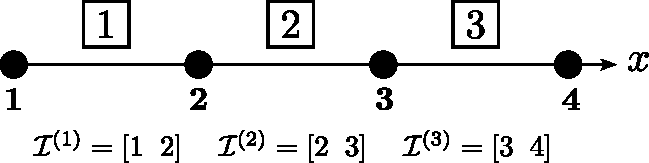
\includegraphics[width=0.6\linewidth]{Figures/IEN_1D.pdf}
	\end{center}
\small
\begin{minipage}{0.5\textwidth}
	\footnotesize
\begin{itemize}
%  \item Connectivity: $\mathcal I^{(1)}=(1,2),\ \mathcal I^{(2)}=(2,3)$
  \item Add the element contributions into the global system::
  \begin{align*}
  K_{ij} &= \sum_e \mathcal{A}_e[\mathbf{K}^{(e)}]_{ij},
  \\
  f_i   &= \sum_e \mathcal{A}_e[\mathbf{f}^{(e)}]_i.
  \end{align*}
  \item Same pattern for any element type (any order $p$, any number of local DOFs).
\end{itemize}
\end{minipage}\hfill
\begin{minipage}{0.45\textwidth}
	\begin{center}
		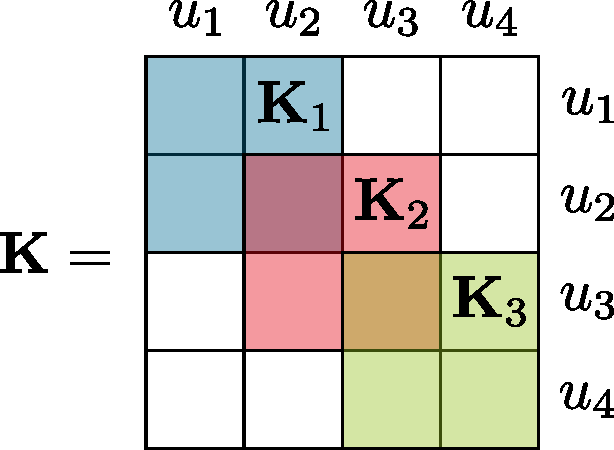
\includegraphics[width=0.75\linewidth]{Figures/Assembly_1D.pdf}
	\end{center}
\end{minipage}
\end{frame}

%====================
\begin{frame}{Assembly for 2D-Problems}
	\begin{minipage}{0.48\textwidth}
		\begin{center}
			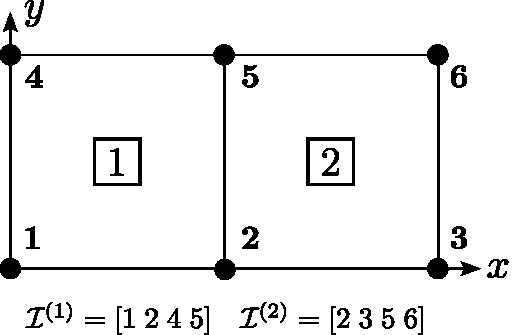
\includegraphics[width=0.98\linewidth]{Figures/Physical_Connectivity_2D.pdf}
		\end{center}
	\end{minipage}\hfill
	\begin{minipage}{0.48\textwidth}
		\textbf{Same idea:}
		\begin{align*}
			K_{ij} &= \sum_e \mathcal{A}_e[\mathbf{K}^{(e)}]_{ij},
			\\
			f_i   &= \sum_e \mathcal{A}_e[\mathbf{f}^{(e)}]_i.
		\end{align*}
	\end{minipage}
	
	\vspace{15pt}
	\begin{minipage}{0.34\textwidth}
		\begin{center}
			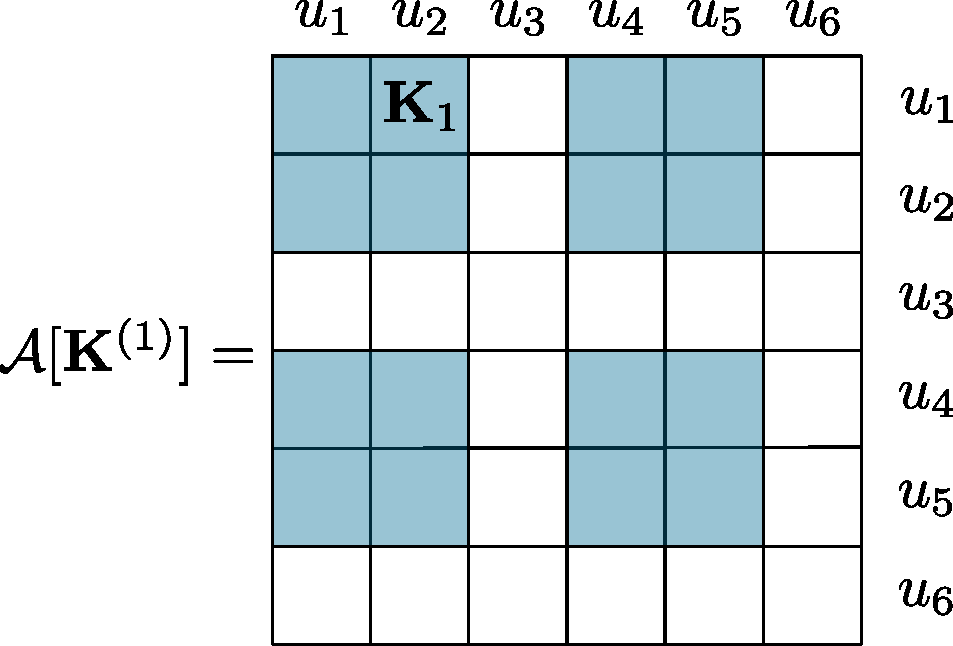
\includegraphics[width=0.98\linewidth]{Figures/Assembly_2D_K1.pdf}
		\end{center}
	\end{minipage}\hfill
	\begin{minipage}{0.34\textwidth}
		\begin{center}
			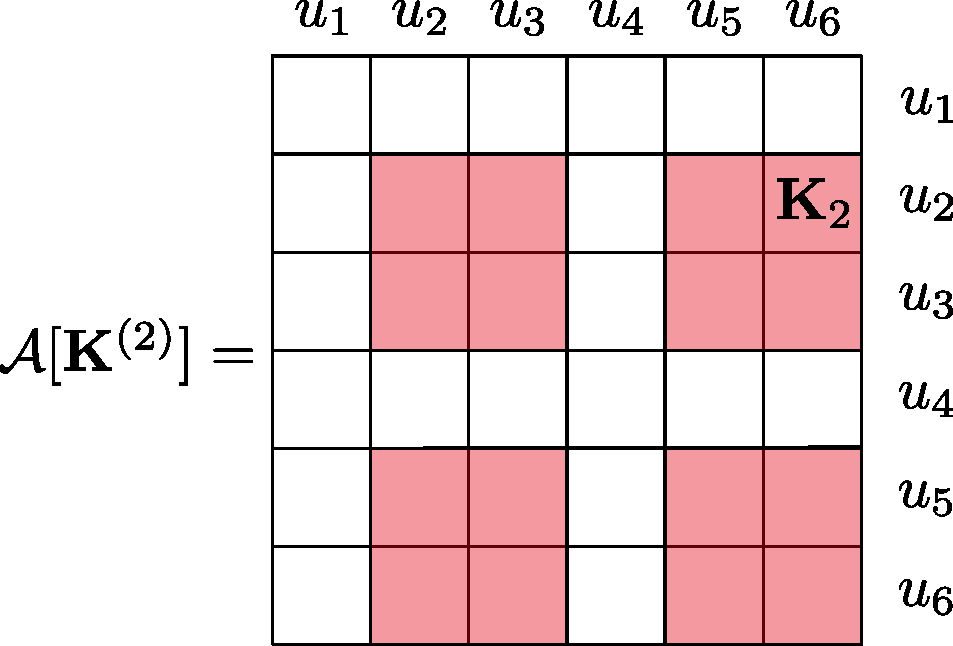
\includegraphics[width=0.98\linewidth]{Figures/Assembly_2D_K2.pdf}
		\end{center}
	\end{minipage}\hfill
	\begin{minipage}{0.29\textwidth}
		\begin{center}
			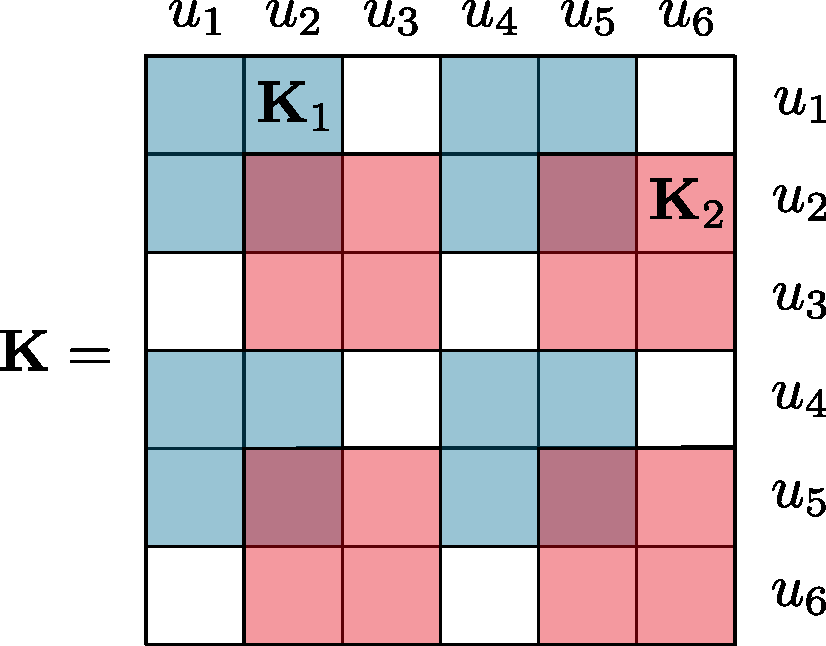
\includegraphics[width=\linewidth]{Figures/Assembly_2D.pdf}
		\end{center}
	\end{minipage}
\end{frame}

%====================
\begin{frame}{Neumann (natural) boundary conditions}
\begin{minipage}{0.5\textwidth}
	\begin{center}
		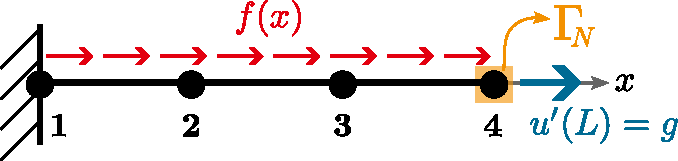
\includegraphics[width=\linewidth]{Figures/Neumann_in_1D.pdf}
	\end{center}
	
	\vspace{20pt}
	\begin{center}
		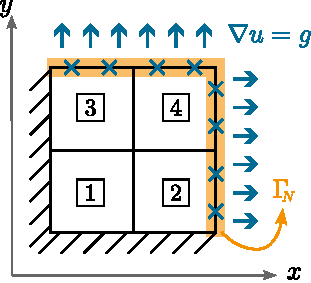
\includegraphics[width=0.7\linewidth]{Figures/Boundary_Integration.pdf}
	\end{center}
	
\end{minipage}\hfill

\begin{minipage}{0.48\textwidth}
		\footnotesize
		\textbf{1D bar (Neumann at $x=L$):}
		\[
		\int_{\Gamma_N} g\,v\,d\Gamma
		\;\Rightarrow\;
		g\,v(L),
		\]
		only the basis function of the node at $L$ is nonzero, so
		\[
		f^{(\Gamma)}_{i_L} \mathrel{+}= g(L)\,N_{i_L}(L) = g(L).
		\]
		
		\vspace{0.7em}
		\textbf{2D (distributed flux on an edge $\Gamma_N$):}
		\[
		t^{(e,\Gamma)}_a \approx \sum_q w_q\, g(\mathbf{x}_q)\,
		N_a(\xi_q,\eta_q)\,
		J_\Gamma(\xi_q,\eta_q),
		\]
		with the \emph{edge} Jacobian
		\[
		J_\Gamma(\xi_q,\eta_q)
		= \Bigl\|\frac{\partial \mathbf{x}}{\partial s}(\xi_q,\eta_q)\Bigr\|,
		\]
\end{minipage}


\end{frame}



\begin{frame}{Dirichlet (essential) boundary conditions}
	\begin{minipage}{0.44\textwidth}
		\begin{center}
			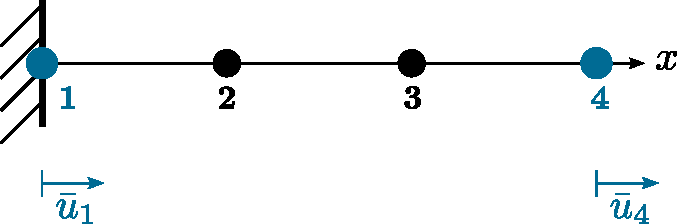
\includegraphics[width=0.98\linewidth]{Figures/pure_Dirichlet_1D.pdf}
		\end{center}
	\end{minipage}\hfill
	\begin{minipage}{0.5\textwidth}
		\small
		\textbf{General idea}
		
		\footnotesize
		Split unknowns into free and prescribed DOFs:
		\[
		\mathbf{U} =
		\begin{bmatrix}
			\mathbf{U}_f \\
			\mathbf{U}_d
		\end{bmatrix},\quad
		\mathbf{K} =
		\begin{bmatrix}
			\mathbf{K}_{ff} & \mathbf{K}_{fd} \\
			\mathbf{K}_{df} & \mathbf{K}_{dd}
		\end{bmatrix},\quad
		\mathbf{f} =
		\begin{bmatrix}
			\mathbf{f}_f \\
			\mathbf{f}_d
		\end{bmatrix}.
		\]
		
		The global system becomes:

		\[
		\mathbf{K}_{ff}\,\mathbf{U}_f
		= \mathbf{f}_f - \mathbf{K}_{fd}\,\bar{\mathbf{U}}_d.
		\]
	\end{minipage}
	
	\vspace{3pt}
	\footnotesize
	\textbf{Example:}
	\vspace{-3pt}
	\[
	\mbox{Original system:   }
	\mathbf{U} =
	\begin{bmatrix}
		\bar u_1 \\[2pt]
		u_2 \\[2pt]
		u_3 \\[2pt]
		\bar u_4
	\end{bmatrix},\quad
	\mathbf{K} =
	\begin{bmatrix}
		K_{11} & K_{12} & K_{13} & K_{14} \\
		K_{21} & K_{22} & K_{23} & K_{24} \\
		K_{31} & K_{32} & K_{33} & K_{34} \\
		K_{41} & K_{42} & K_{43} & K_{44}
	\end{bmatrix},\quad
	\mathbf{f} =
	\begin{bmatrix}
		f_1 \\[2pt] f_2 \\[2pt] f_3 \\[2pt] f_4
	\end{bmatrix}.
	\]
	

	\[
	\mbox{Reduced system:   }\underbrace{
		\begin{bmatrix}
			K_{22} & K_{23} \\
			K_{32} & K_{33}
	\end{bmatrix}}_{\mathbf{K}_{ff}}
	\begin{bmatrix}
		u_2 \\[2pt] u_3
	\end{bmatrix}
	=
	\underbrace{
		\begin{bmatrix}
			f_2 \\[2pt] f_3
	\end{bmatrix}}_{\mathbf{f}_f}
	-
	\underbrace{
		\begin{bmatrix}
			K_{21} & K_{24} \\
			K_{31} & K_{34}
	\end{bmatrix}}_{\mathbf{K}_{fd}}
	\begin{bmatrix}
		\bar u_1 \\[2pt] \bar u_4
	\end{bmatrix}.
	\]
\end{frame}



\begin{frame}{Wrap-up: Practical Notes and Outlook}
	\small
	\textbf{Practical checklist}
	\begin{itemize}
		\item Consistent element connectivity and boundary edge orientation.
		\item Correct use of the Jacobians for the volume and boundary integrals.
		\item Make sure outward normals are consistent on Neumann boundaries.
%		\item Choose quadrature order consistent with the polynomial degree.
		\item After applying Dirichlet BCs, solve only for the free DOFs.
	\end{itemize}
	
	\vspace{0.5em}
	\textbf{Outlook: link to machine learning for scientific computations}
	\begin{itemize}
		\item In PINNs, PDE residuals and boundary conditions can appear directly in the loss function.
		\item Neural Operators are often trained on data generated by FEM solvers assembled in this way.
	\end{itemize}
\end{frame}


\end{document}
